% Options for packages loaded elsewhere
\PassOptionsToPackage{unicode}{hyperref}
\PassOptionsToPackage{hyphens}{url}
%
\documentclass[
  12 pt,
  a4paper,
]{article}
\usepackage{amsmath,amssymb}
\usepackage{setspace}
\usepackage{iftex}
\ifPDFTeX
  \usepackage[T1]{fontenc}
  \usepackage[utf8]{inputenc}
  \usepackage{textcomp} % provide euro and other symbols
\else % if luatex or xetex
  \usepackage{unicode-math} % this also loads fontspec
  \defaultfontfeatures{Scale=MatchLowercase}
  \defaultfontfeatures[\rmfamily]{Ligatures=TeX,Scale=1}
\fi
\usepackage{lmodern}
\ifPDFTeX\else
  % xetex/luatex font selection
  \setmainfont[]{Times New Roman}
\fi
% Use upquote if available, for straight quotes in verbatim environments
\IfFileExists{upquote.sty}{\usepackage{upquote}}{}
\IfFileExists{microtype.sty}{% use microtype if available
  \usepackage[]{microtype}
  \UseMicrotypeSet[protrusion]{basicmath} % disable protrusion for tt fonts
}{}
\makeatletter
\@ifundefined{KOMAClassName}{% if non-KOMA class
  \IfFileExists{parskip.sty}{%
    \usepackage{parskip}
  }{% else
    \setlength{\parindent}{0pt}
    \setlength{\parskip}{6pt plus 2pt minus 1pt}}
}{% if KOMA class
  \KOMAoptions{parskip=half}}
\makeatother
\usepackage{xcolor}
\usepackage[margin=1in]{geometry}
\usepackage{graphicx}
\makeatletter
\def\maxwidth{\ifdim\Gin@nat@width>\linewidth\linewidth\else\Gin@nat@width\fi}
\def\maxheight{\ifdim\Gin@nat@height>\textheight\textheight\else\Gin@nat@height\fi}
\makeatother
% Scale images if necessary, so that they will not overflow the page
% margins by default, and it is still possible to overwrite the defaults
% using explicit options in \includegraphics[width, height, ...]{}
\setkeys{Gin}{width=\maxwidth,height=\maxheight,keepaspectratio}
% Set default figure placement to htbp
\makeatletter
\def\fps@figure{htbp}
\makeatother
\setlength{\emergencystretch}{3em} % prevent overfull lines
\providecommand{\tightlist}{%
  \setlength{\itemsep}{0pt}\setlength{\parskip}{0pt}}
\setcounter{secnumdepth}{-\maxdimen} % remove section numbering
\ifLuaTeX
\usepackage[bidi=basic]{babel}
\else
\usepackage[bidi=default]{babel}
\fi
\babelprovide[main,import]{spanish}
\ifPDFTeX
\else
\babelfont{rm}[]{Times New Roman}
\fi
% get rid of language-specific shorthands (see #6817):
\let\LanguageShortHands\languageshorthands
\def\languageshorthands#1{}
\ifLuaTeX
  \usepackage{selnolig}  % disable illegal ligatures
\fi
\usepackage{bookmark}
\IfFileExists{xurl.sty}{\usepackage{xurl}}{} % add URL line breaks if available
\urlstyle{same}
\hypersetup{
  pdflang={es-ES},
  hidelinks,
  pdfcreator={LaTeX via pandoc}}

\title{U8 VIRTUALITZACIÓ WINDOWS 11}
\usepackage{etoolbox}
\makeatletter
\providecommand{\subtitle}[1]{% add subtitle to \maketitle
  \apptocmd{\@title}{\par {\large #1 \par}}{}{}
}
\makeatother
\subtitle{Comunicació amb la màquina amfitriona}
\author{}
\date{\vspace{-2.5em}}

\begin{document}
\maketitle

\setstretch{1.5}
\newpage
\renewcommand\tablename{Tabla}

\begin{center}\rule{0.5\linewidth}{0.5pt}\end{center}

A la Unitat 2 teniu més informació sobre VirtuaBox. Ara anem a provar
algunes configuracions que afecten a la \textbf{comunicació entre la
nostra màquina virtual Windows 11 i l'amfitrió}.

\section{La tarja de xarxa (NIC)}\label{la-tarja-de-xarxa-nic}

Al mòdul de Xarxes Locals veieu el que és la tarja i que té una IP.
També estudiareu les IPs, els rangs, famílies\ldots{}

Ací vorem les formes de configurar la targeta d'una màquina virtual.

\subsection{Adaptador pont}\label{adaptador-pont}

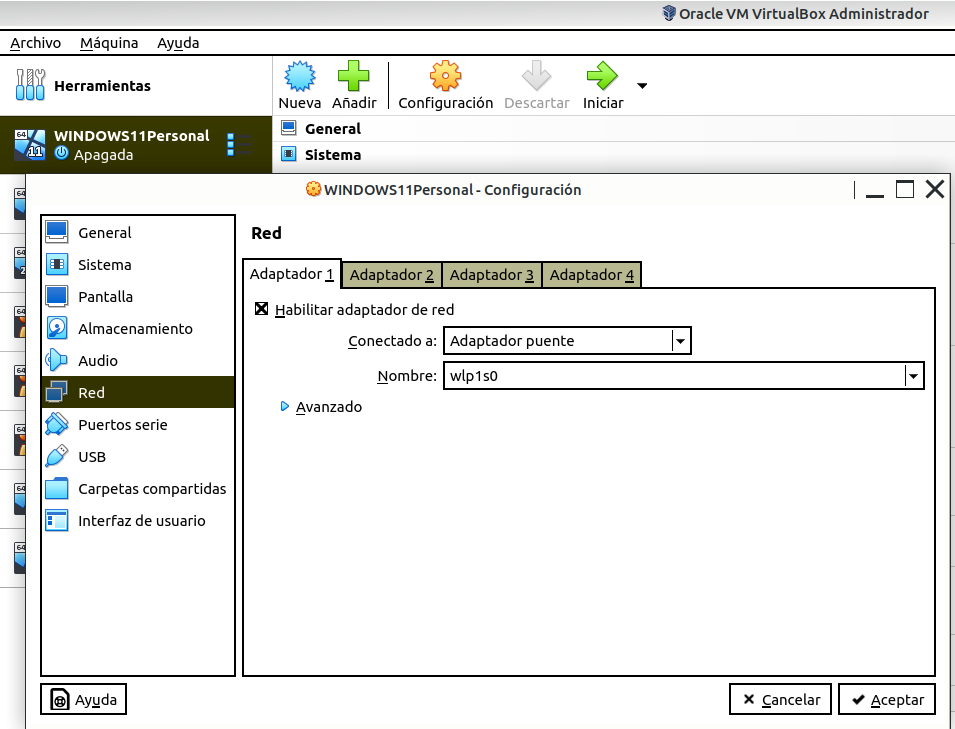
\includegraphics{png/adaptadorpont.png}

\begin{itemize}
\item
  Tindrà un IP de la mateixa família que el PC amfitrió.
\item
  Si el PC té internet (WIFI, cable o mòbil), la màquina virtual també.
\item
  Heu de comprovar que les ip son de la mateixa família fent
  \textbf{ipconfig}. En la màquina física i en la virtual.
\item
  Feu un ping entre les dos ip.
\end{itemize}

WIN + R, CMD, ipconfig

\subsection{NAT}\label{nat}

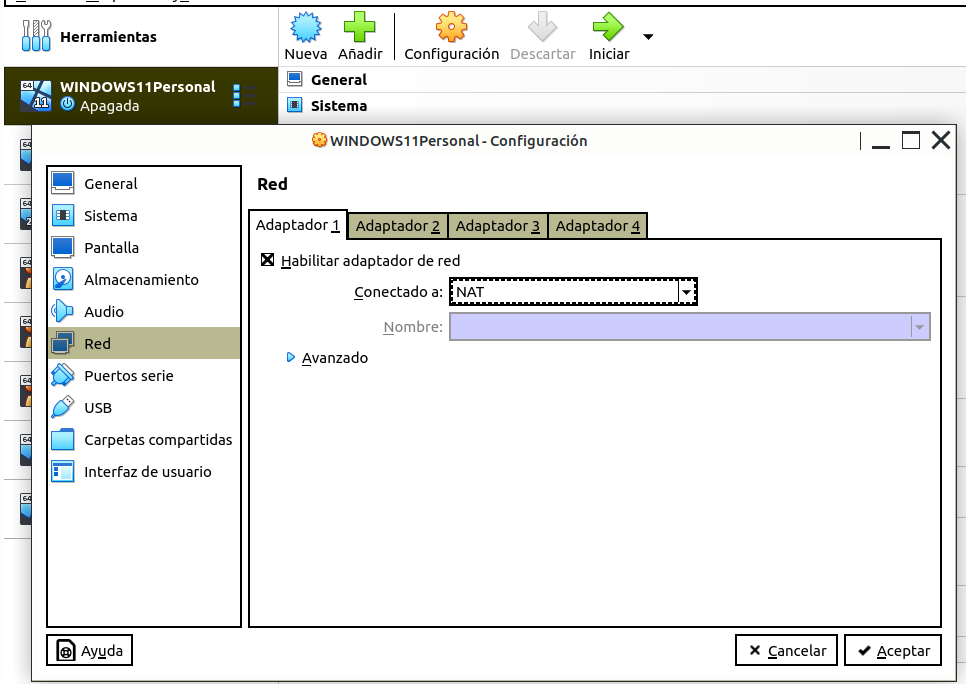
\includegraphics{png/NAT.png}

La ip de la màquina virtual serà d'una altra família a la de la màquina
real però hi haurà una ``traducció''. Esta traducció és similar a la que
fa el vostre router a casa entre ip pública i ip privada. Per tant, si
el PC o portàtil té internet, esta màquina virtual, també.

\begin{itemize}
\tightlist
\item
  Heu de comprovar que les ip NO son de la mateixa família fent
  \textbf{ipconfig} En la màquina física i en la virtual.
\item
  Feu un ping entre les dos ip
\end{itemize}

WIN + R, CMD, ipconfig

\subsection{Xarxa interna}\label{xarxa-interna}

La ip de la màquina virtual serà d'una altra família a la de la màquina
real i no hi ha cap ``traducció''.

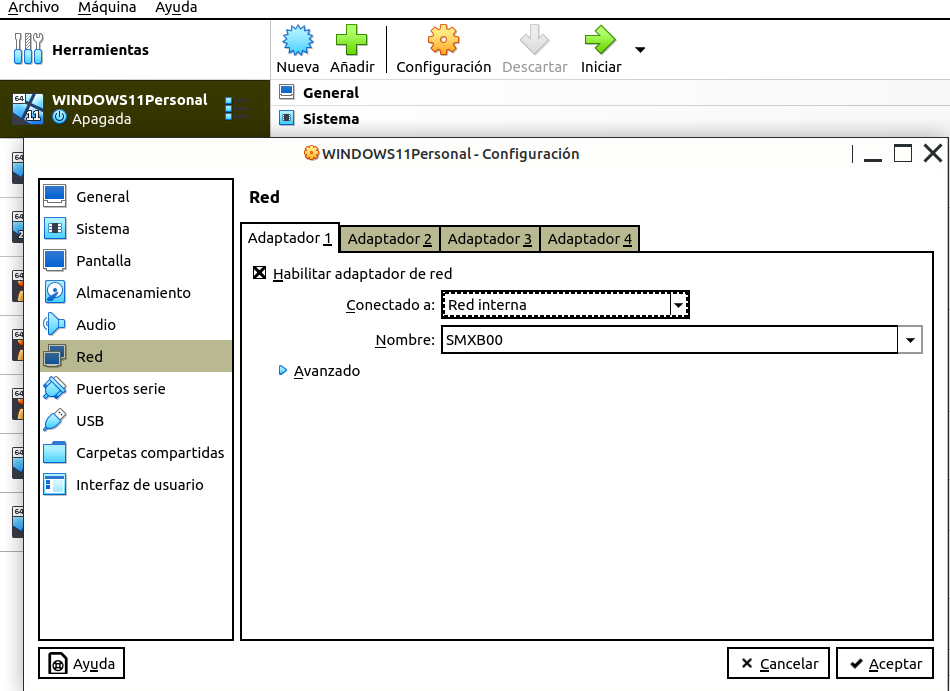
\includegraphics{png/xarxainterna.png}

\begin{itemize}
\tightlist
\item
  Heu de comprovar que les ip NO son de la mateixa família fent
  \textbf{ipconfig} En la màquina física i en la virtual.
\item
  Feu un ping entre les dos ip. No es comunicaran
\end{itemize}

En esta configuració les màquines virtuals estan aïllades de la real.

\newpage

\section{Carpetes compartides}\label{carpetes-compartides}

En \textbf{Dispositius}

No s'ha de confondre amb la compartició de fitxers i carpetes en xarxes
locals que es veu més avant. Ací només es tracta de que, des de la MV es
puga accedir una carpeta de l'amfitrió.

Podem triar si volem:

\begin{itemize}
\item
  Sols de lectura.
\item
  Fer permanent. Per a que, en reiniciar, estiga disponible.
\end{itemize}

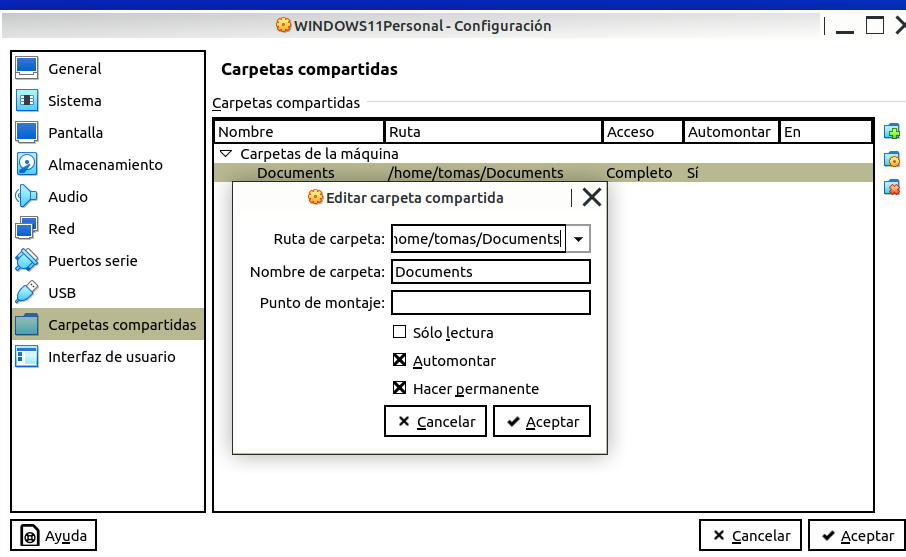
\includegraphics{png/carpetacompartida.png}

Ara ja vorem en el nostre explorardor de la Màquina virtual la carpeta
de la màquina amfitriona.

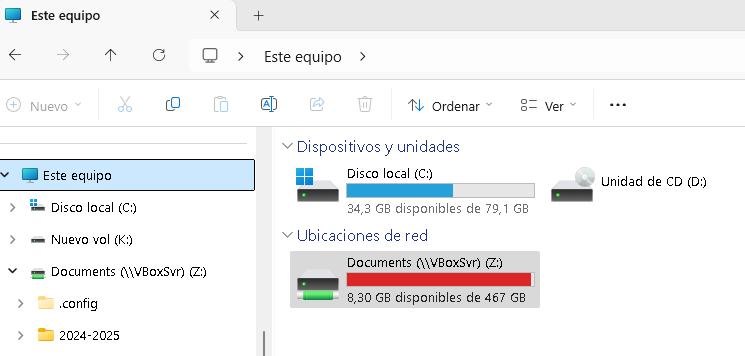
\includegraphics{png/explorador.png}

\textbf{Ús habitual}

Si treballem en un Lubuntu a casa pero el nostre portàtil és un Windows
Home, molt probablement voldrem que els documents o imatges ( captures
de pantalla de les pràctiques, per exemple) es guarden a Documentos del
Windows. Compartiríem esta carpeta de Windows en el Lubuntu.

\newpage

\section{Copiar entre màquines.}\label{copiar-entre-muxe0quines.}

En \textbf{Dispositius}

\subsubsection{Portapapers}\label{portapapers}

Si volem fer CONTROL + C i CONTROL + V entre les 2 màquines
(Portapapeles)

o si volem

\subsubsection{``arrastrar y soltar''}\label{arrastrar-y-soltar}

Les opcions per habilitar-ho són:

\begin{itemize}
\tightlist
\item
  Inhabilitat.
\item
  Només per a copiar des de l'amfitrió a la virtual.
\item
  Només per a copiar des de la virtual a l'amfitrió.
\item
  Bidireccional
\end{itemize}

\end{document}
